\documentclass[tikz,border=10pt]{standalone}
\usepackage{tkz-euclide} % 用于方便地获取点和标注直角

\begin{document}
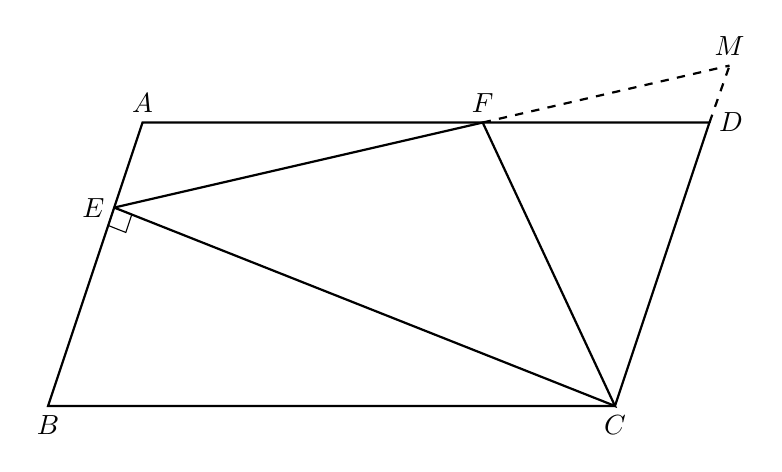
\begin{tikzpicture}[scale=1.2, >=stealth]
    % 1. 定义平行四边形的顶点 (设置坐标以符合图片视觉比例)
    \coordinate (A) at (1, 3);
    \coordinate (B) at (0, 0);
    \coordinate (C) at (6, 0);
    \coordinate (D) at (7, 3);

    % 2. 定义内部点 E 和 F
    % E 在 AB 上, F 在 AD 上
    \coordinate (E) at ($(A)!0.3!(B)$);
    \coordinate (F) at ($(A)!0.6!(D)$);

    % 3. 定义垂直点（或根据视觉模拟 C 与 EF 的关系）
    % 为了符合图像中的直角表现，我们直接连接 EC 与 FC
    % M 是 EF 延长的点
    \coordinate (M) at ($(E)!1.67!(F)$);

    % 4. 绘制实线部分
    \draw[thick] (A) -- (B) -- (C) -- (D) -- cycle; % 平行四边形轮廓
    \draw[thick] (E) -- (F) -- (C) -- (E);         % 内部三角形/折线

    % 5. 绘制虚线部分
    \draw[thick, dashed] (F) -- (M);
    \draw[thick, dashed] (D) -- (M);

    % 6. 绘制直角符号 (角 FEC)
    \tkzMarkRightAngle[size=0.2](C,E,B)

    % 7. 标注字母标签
    \node[above] at (A) {$A$};
    \node[below] at (B) {$B$};
    \node[below] at (C) {$C$};
    \node[right] at (D) {$D$};
    \node[left] at (E) {$E$};
    \node[above] at (F) {$F$};
    \node[above] at (M) {$M$};

\end{tikzpicture}
\end{document}